 \documentclass[11pt,a4paper]{article}
\usepackage[utf8]{inputenc}		% LaTeX, comprend les accents !
\usepackage[T1]{fontenc}
\usepackage{natbib}	
%\usepackage[square,sort&compress,sectionbib]{natbib}		% Doit être chargé avant babel      
\usepackage[frenchb,english]{babel}
\usepackage{lmodern}
\usepackage{amsmath,amssymb, amsthm}
\usepackage{a4wide}
\usepackage[capposition=top]{floatrow}
\usepackage{verbatim}
\usepackage{float}
\usepackage{placeins}
\usepackage{flafter}
\usepackage{longtable}
\usepackage{import}
\usepackage{pdflscape}
\usepackage{rotating}
\usepackage{hhline}
\usepackage{multirow}
\usepackage{booktabs}
\usepackage[pdftex,pdfborder={0 0 0},colorlinks=true,linkcolor=blue,urlcolor=blue,citecolor=blue,bookmarksopen=true]{hyperref}
\usepackage{eurosym}
%\usepackage{breakcites}
\usepackage[autostyle]{csquotes}
%\usepackage{datetime}
\usepackage{natbib}
\usepackage{setspace}
\usepackage{lscape}
\usepackage[usenames]{color}
\usepackage{indentfirst}
\usepackage{url}
\usepackage{enumitem}
\usepackage{multirow}
\usepackage{subcaption}
\usepackage[justification=centering]{caption}
\bibliographystyle{agsm}
\usepackage{supertabular} 
\usepackage{array}
\usepackage{longtable}
\newcommand{\isEmbedded}{true}

\graphicspath{{Figures/}}


\begin{document}

\selectlanguage{frenchb}
\title{Le corps : bon niveau de la modélisation ?}


\author{}


\maketitle

\section{Effectifs par corps en 2012.}

\begin{table}[h!]
	\label{means}
	\centering
	\caption{Nombre d'agents par corps en 2012} 
\begin{tabular}{llr}
	\toprule
	{} &                                Label corps en 2012 &  Nombre agents \\
	\midrule
	0  &                      Agents technique territoriaux &         376323 \\
	1  &                                    Aides soignants &         174226 \\
	2  &               Adjoints administratifs territoriaux &         163009 \\
	3  &        Infirmiers en soins generaux et specialises &         122260 \\
	4  &                                         Infirmiers &          80796 \\
	5  &         Agents des services hospitaliers qualifies &          64585 \\
	6  &  Agents territoriaux specialises des ecoles mat... &          32011 \\
	7  &               Adjoints administratifs hospitaliers &          31612 \\
	8  &                               Adjoints d animation &          27419 \\
	9  &                            Ouvriers professionnels &          23954 \\
	10 &                                 Agents d entretien &          13735 \\
	11 &                        Agents sociaux territoriaux &          13623 \\
	12 &                               Secretaires medicaux &          13599 \\
	13 &                    Agents de maitrise territoriaux &          13442 \\
	14 &          Assistants territoriaux sociaux educatifs &          13173 \\
	15 &                           Techniciens territoriaux &           9652 \\
	16 &                                      Contremaitres &           2760 \\
	17 &      Sapeurs pompiers professionnels non officiers &           1219 \\
	18 &                              Attaches territoriaux &             70 \\
	19 &                            Ingenieurs territoriaux &             13 \\
	20 &                                   Maitres Ouvriers &             13 \\
	\bottomrule
\end{tabular}
\begin{minipage}{15cm}
	\footnotesize
	\textsc{Population:} Individus qui ont leur code grade NEG renseigné pour l'année 2012 (1 253 937 identifiants) 1 177 494 agents sont représentés dans le tableau et 76 443 individus sont dans un corps sans label en 2012, c'est-à-dire qu'ils appartiennent aux grades suivants : S09886, N00466, S08733, S05490, S10067, S04395 pour lesquels on n'a pas de corps dans le fichier $corresp\_{}neg\_{}netneh.csv$. 67 agents ont plusieurs code grades pour l'année 2012\\
\end{minipage}
\end{table}





% Section I: Analyse des grilles
\section{Transitions intra-corps entre 2012 et 2013.}


On veut savoir si les transitions de carrières se font majoritairement à l'intérieur des corps, et si ces caractéristiques des transitions de carrières concernent tous les corps de façon égale.


\subsection{Echantillon des individus qui ont leur code grade renseigné en 2012 et en 2013.}

Sur la figure 1, on voit que beaucoup d'agents qui sont dans un corps en 2012 le sont aussi en 2013. Toutefois, si on restreint l'échantillon aux agents qui changent de grade entre 2012 et 2013 (figure 2), on voit d'une part qu'il y a moins d'adhérence au corps de façon générale et d'autre part que l'adhérence au corps dépend du corps. En effet, certains corps retiennent davantage les agents changeant de grades (tels les adjoints techniques territoriaux avec 90 \% de rétention de ces personnes) que d'autres corps (tels les agents de maîtrise territoriaux, qui ne retiennent qu'environ 40 \% des personnes changeant de grade entre 2012 et 2013).

\begin{figure}[H] 
	\caption{Parts des agents restant dans un même corps entre 2012 et 2013, par corps en 2012.}
	\label{transit1} 
	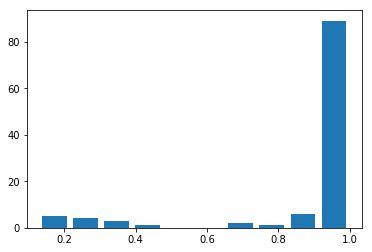
\includegraphics[scale = 0.7]{transitions_intra_corps_2012_2013.png} 
\begin{minipage}{15cm}
	\footnotesize
	\textsc{Population:} Individus qui ont leur code grade NEG renseigné pour les deux années 2012 et 2013 (1 126 480 identifiants). 1 112 332 agents restent dans un même corps entre 2012 et 2013. 21 corps sont représentés.\\
	\textsc{Lecture:} Dans 9 corps sur 21, environ 100 \% des personnes qui étaient dans un corps en 2012 restent dans ce même corps en 2013. \\
	\textsc{Note:} Les deux corps qui ont le plus faible taux de rétention à l'intérieur de leur corps (environ 0.92) sont les agents d'entretien et les agents sociaux territoriaux.
\end{minipage}
\end{figure}


\begin{figure}[H] 
	\caption{Parts des agents changeant de grade entre 2012 et 2013 et restant dans un même corps entre 2012 et 2013, par corps en 2012.}
	\label{transit2} 
	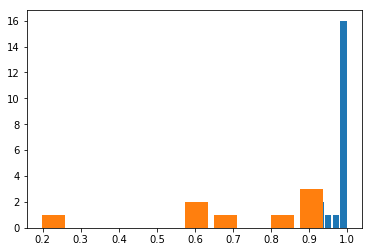
\includegraphics[scale = 0.7]{transitions_intra_corps_only_w_c_neg_change_2012_2013.png} 
	\begin{minipage}{15cm}
		\footnotesize
		\textsc{Population:} Individus qui ont leur code grade NEG renseigné pour les deux années 2012 et 2013 et qui changent de code grade NEG entre 2012 et 2013 (91 189 identifiants, soit moins de 10 \% des agents ayant leur grade renseigné pour les deux années). 9 corps sont représentés, car les 12 autres n'ont aucun individu changeant de grade entre 2012 et 2013.\\
		\textsc{Lecture:} Dans 3 corps sur 21, environ 90 \% des personnes qui étaient dans un corps en 2012 et qui changent de grades entre 2012 et 2013 restent dans ce même corps en 2013. \\
		\textsc{Note:} Le corps qui a le plus faible taux de transition de grades internes (environ 0.4) est celui des agents de maîtrise territoriaux. Les corps qui ont les taux de transition de grades internes les plus haut (environ 0.9) sont les adjoints administratifs territoriaux, les adjoints techniques territoriaux et les agents territoriaux des écoles maternelles.
	\end{minipage}
\end{figure}




\end{document}